% !TEX root =  ../main.tex 

\section{Personalized schedules for patients in PRIAS}
\label{sec : pers_schedule_PRIAS}
As a first step in demonstrating how the personalized schedules work, we created a biopsy schedule for patients in PRIAS. To this end, we divided the PRIAS data set into training(5938 subjects) and demonstration data sets (5 subjects). We demonstrate that the biopsy schedule depend on subject specific traits and the evolution of PSA scores.\\ 

\begin{figure}[!htb]
\centering
\captionsetup{justification=centering}
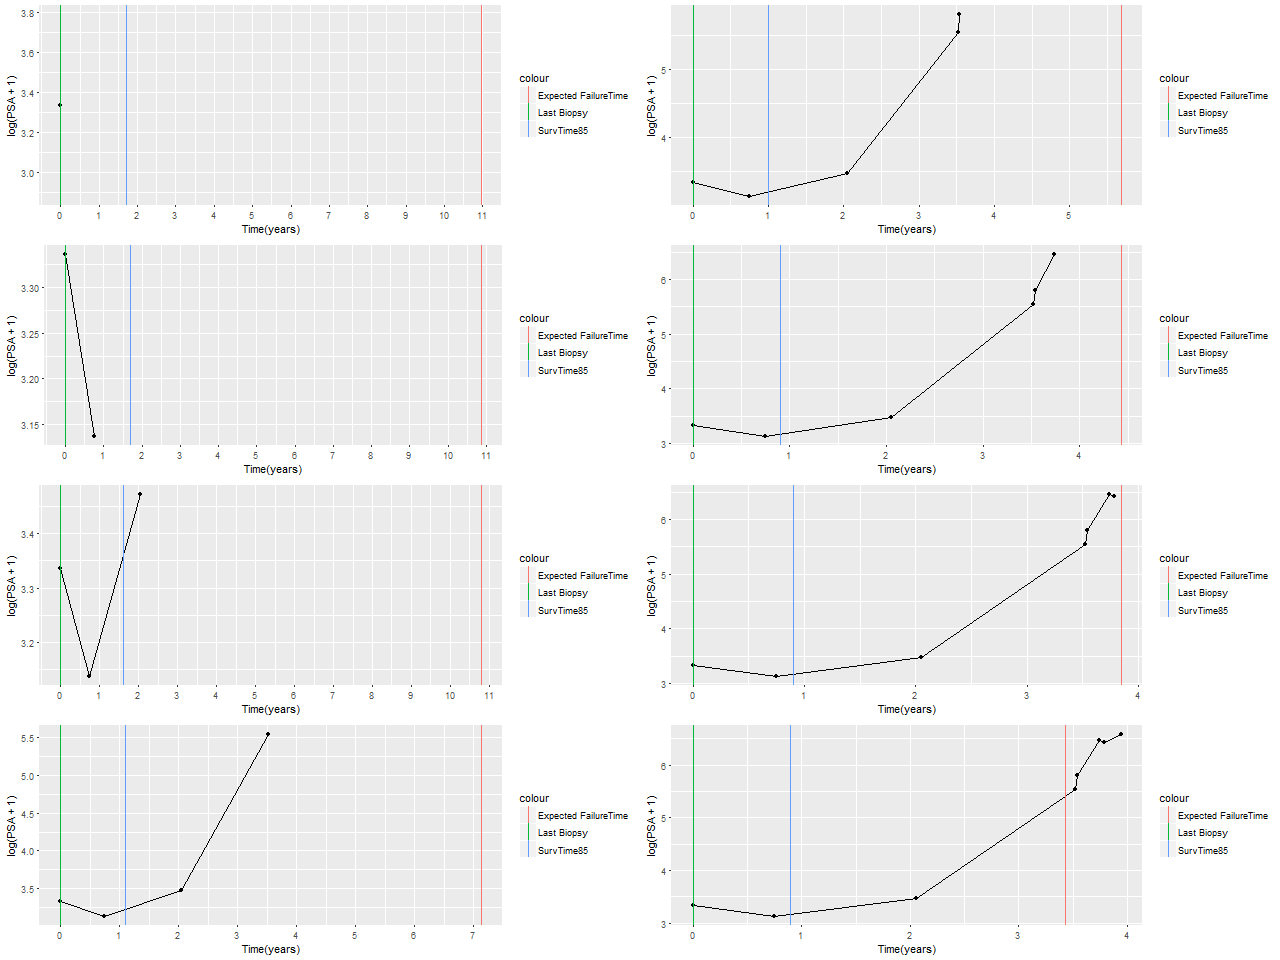
\includegraphics[width=\textwidth]{prias_demo_pid_3174.png}
\caption{\label{fig : prias_demo_pid_3174} Proposed biopsy times for patient 3174 from PRIAS.}
\end{figure}

\begin{figure}[!htb]
\centering
\captionsetup{justification=centering}
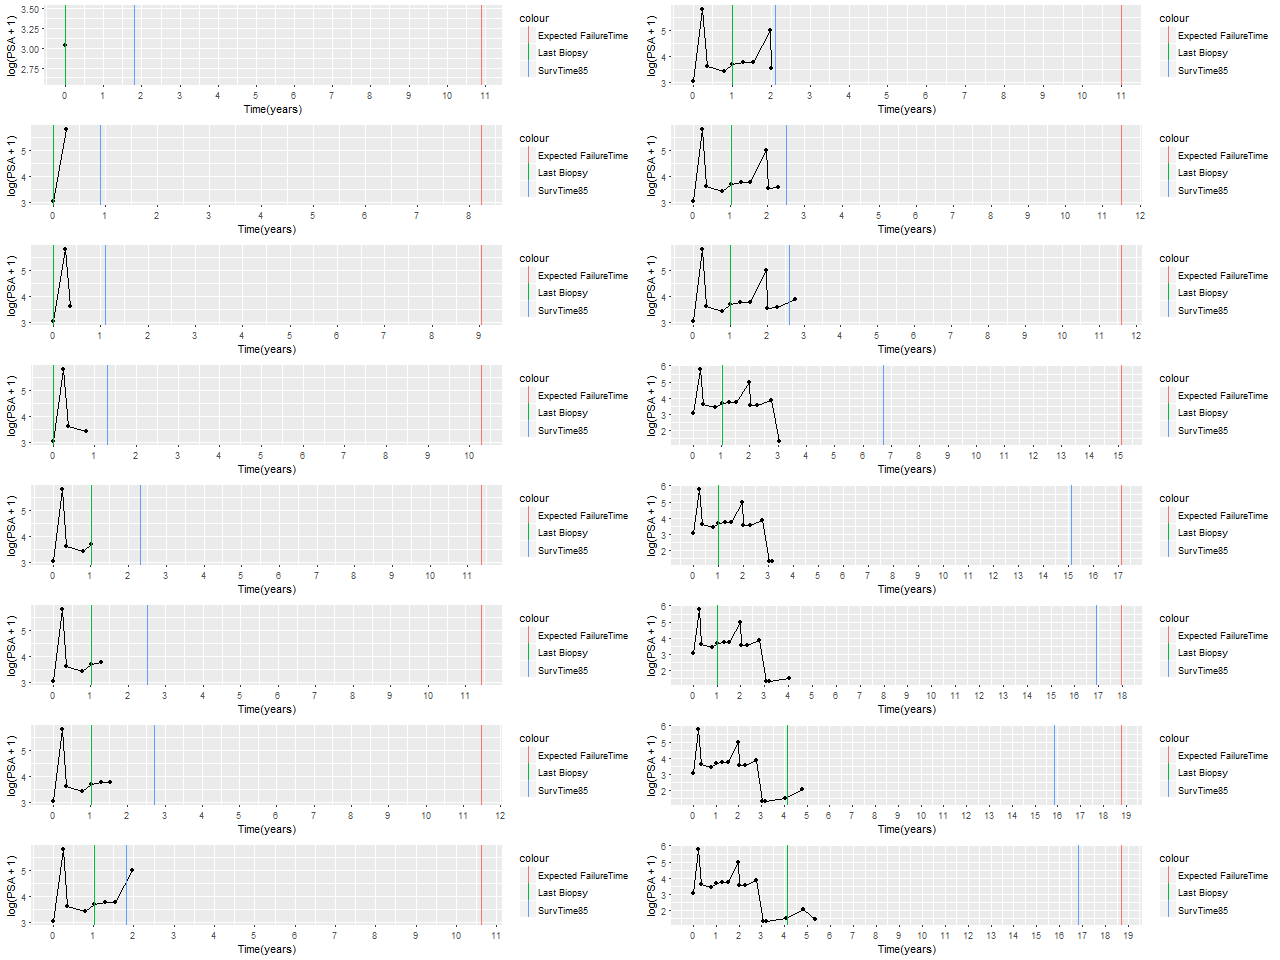
\includegraphics[width=\textwidth]{prias_demo_pid_911.png}
\caption{\label{fig : prias_demo_pid_911} Proposed biopsy times for patient 3174 from PRIAS.}
\end{figure}

\begin{figure}[!htb]
\centering
\captionsetup{justification=centering}
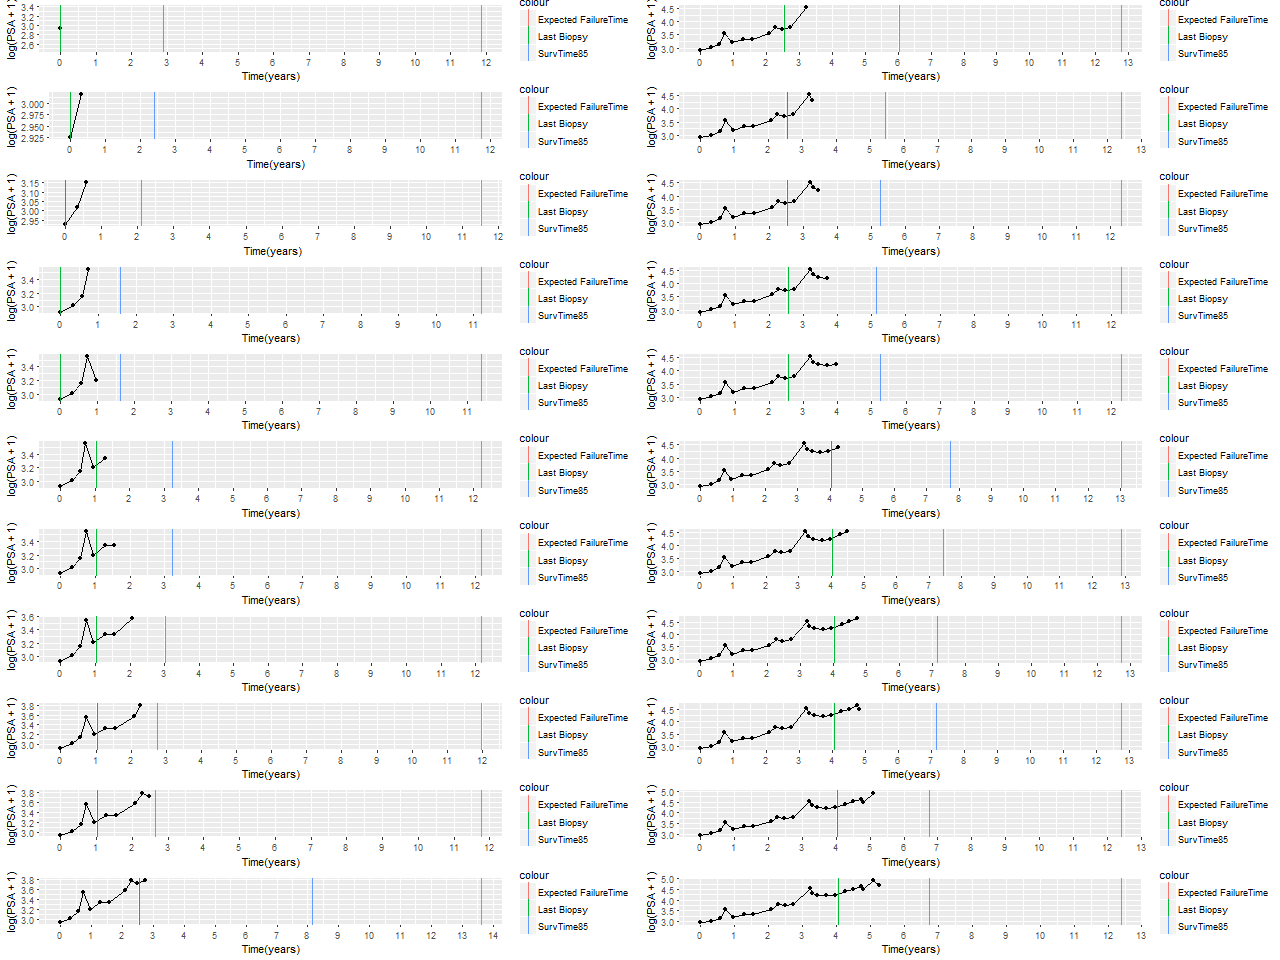
\includegraphics[width=\textwidth]{prias_demo_pid_2340.png}
\caption{\label{fig : prias_demo_pid_2340} Proposed biopsy times for patient 3174 from PRIAS.}
\end{figure}

It can be seen in Figure \ref{fig : prias_demo_pid_3174} that the patient 3174 had a biopsy at the time of induction and none after that. The PSA for the patient increases rapidly after the 2nd year. In response to this rapid increase, the proposed biopsy times based on conditional expected failure time also decrease accordingly from 11 years to around 3.4 years. The change for risk based methods is not so drastic though. Further it can be seen that at the last visit for PSA, the proposed biopsy time is earlier than the last 5 PSA visits and similar is the case for the proposed biopsy time based on dynamic risk of failure. This is due to the fact that the last time of biopsy was time 0 (induction time) and thus the time to Gleason reclassification can take any value larger than 0. We discuss this issue in detail in section \ref{subsec : simulation_setup}.\\

Figure \ref{fig : prias_demo_pid_911} shows the PSA evolution and biopsy times for subject 911. It can be seen that this patient had 3 biopsies where Gleason reclassification did not happen. At year 2 when the patient's PSA increases rapidly the proposed failure times also decrease, whereas they increase over the next 1 year because the PSA also drops down in that time period. The fact that PSA velocity affects the biopsy times the most is also evident in the case of subject 2340, whose evolution is shown in Figure \ref{fig : prias_demo_pid_2340}. Here the rate of change at each time point is not high, and even though the PSA value reaches as high as 25 it has no effect on proposed biopsy times. This is in accordance with the estimated strength of association between PSA velocity/value and hazard of time to Gleason reclassification.\\

An interesting observation we made while creating these schedules was that the variance of time to Gleason reclassification (Eq. \ref{eq : varFailureTime}) was quite high, which essentially rules out the usefulness of conditional expected time to Gleason reclassification. Given the large difference in proposed biopsy times based on the former and methods based on dynamic risk of Gleason reclassification, one might conclude that the latter are more useful. However as we will see in the simulation study (Section \ref{sec: simulation_study}) ahead, the usefulness of the two categories of methods depends on the distribution of time to Gleason reclassification.
